\section{Literature Review}~\label{sec:literature}

\todojc{You do not need to say what lit reviews are}This section aims to gain an understanding of the use of classical and quantum methods in signal processing in \ac{EW}.

% Search Strategy
\todojc{I've changed this, you need to say these uninteresting things in a simple way}The review of the relevant concepts and methods was supported with library search tools (cf. search terms in Section \ref{sec:appendix1}), Google Scholar, selected books and journals related to quantum computing and signal processing. 
\todo{cite: these resources}

% Selection criteria
\todojc{As I said before, the scope of your lit review is not any different from the scope of your research, so move all of these to the "Scope" section}Study selection criteria will be used to determine which studies are included or excluded from the review.
% Scope
The scope of review will be used to screen studies on a per-study basis based on the whether it meets a criteria for inclusion, or exclusion.

\begin{itemize}
    \item Hardware - neither the physical implementation's of quantum nor radar will be considered.
    \item \ac{ESM}-focused. Only digitised signals to parameter estimation will be examined. Anything down-stream of identification of radar signals, (e.g., display, databasing, data fusion, etc.) and before digitisation (receive path, antennas, etc.) will be excluded
    \item \ac{SAR} and imaging radar functions
    \item Kinetic and located radar systems:
    \begin{itemize}
        \item Multi-path effects
        \item Located antennas - bi-static/multi-static, arrays
        \item Range, velocity, angle of arrival, etc.
    \end{itemize}
    \item Radar emission. Only passive, or pure \ac{ESM} scenarios will be considered
    \item Detailed radar simulation will be excluded.
    \item The range of frequency to be considered will fall within \(50MHz - 50GHz\) and be exclusive of communications signals.
    \item Adjacent problems in radar will be granted limited attention:
    \begin{itemize}
        \item Resource allocation
        \item Ambiguity analysis
        \item Tracking
    \end{itemize}
\end{itemize}

%%%%%%%%%%%%%%%%
%% Begin narrative Meta-analysis review
% Quality assesment checklist
A quality assessment checklist \cite{kitchenham_can_2010} has been adopted in order to \todojc{I've removed "quantitatively", as the assessment is rather "qualitative", also the fact that they used it for SE is not relevant, so it was removed}assess the studies based on their methodological completeness(see evaluation aspects in \ref{sec:appendix2}). 

% Meta-analysis
\todojc{Has this be done? If so add such tables to the appendix and cross-ref from here}A formal meta-analysis will be conducted, and tables \todojc{Has been?}\textbf{will be} created to highlight similarities and differences among the studies.
% Classification
Each study is categorised by the \emph{topic} selected from the following list.
% Not sure if I must list them
\begin{itemize}
    \item Signal processing
    \item Time-series analysis
    \item Quantum time-series analysis
    \item Quantum encoding
    \item Quantum techniques
    \item \ac{EW}
    \item Radar techniques
    \item Radar fundamentals
\end{itemize}

The studies are also classified by the \emph{methodology} used \cite{wohlin_empirical_2012}.
\begin{itemize}
    \item Survey
    \item Case study
    \item Experimental
    \item Quasi-experimental
\end{itemize}

\todo{I have a table, but It seems really verbose to paste it here. It's also quite large and won't fit... see attachment 'Literature Review.xlsx'. This is effectively the meta-analysis}
\todojc{Put an improved table in the Appendix A/B/C...}
\todo{Put some stats here}

%%%%%%%%%%%%%%%%
%%% Begin narrative synthesis
%% Questions to ask:
% What is the aim of the paper?
% What are the main contributions of the paper? What new ideas are presented?
% How is the research contribution or claims justified?
% What sorts of experiments were conducted and how were the experiments set up?
% What data was obtained and how does it justify the claims made?
% Were the experiments adequate? Did they gather enough data to support the claims?
% Was data interpreted correctly? Or, Is there any explicit or hidden bias?
% Was the reasoning in the paper sound?
% What were the assumptions made in the research? Are the assumptions valid or realistic?
% How new or significant is the research idea or contribution? What are the implications to the field of the research presented?
% What are the novel aspects of the work?
% What are the shortcomings of the work? What are strengths and weakness?
% How can the work be extended or shortcomings dealt with? Does the paper encourage future work in the area?
% Are the results generalisable or applicable to another context? Are there improvements that could be made on the work?
% How is the paper relevant to your research, and how does it link to previous papers you’ve read?
%%%%%%%%%%%%%%%%

\subsection{Radar Signal Processing}
%% The problem of radar / EW
As has been illustrated, the complexity of the \ac{ESM} signal environment warrants equally complex answers to understanding it.
% Grand challenges in radar sig. proccessing / Four Problems in Radar
F. Gini \cite{gini_grand_2021} and M. Wicks and B. Himed \cite{wicks_four_2004} attempt to survey such challenges and future solutions. 
% Critique
Each survey satisfactorily outlines the challenges in the field of radar and signal processing, providing an illustrative overview of the emerging fields in radar engineering - waveform design, signal processing, and \ac{STAP}.
% Argument
The authors agree on a number of unanswered questions:
% Questions - not a big fan of enumerating them here.
% Q1
How to design distributed \ac{MIMO} radar to maximize detection performance and coverage area, while minimizing the revisit rate.
% Q2
How to use algorithmic hypothesis testing to merge detection and parameter estimation algorithms.
% Q3
How to better detect targets in the presence of noise and clutter by combining knowledge of signal characteristics and geometric factors.
% Q4
How to create a develop a framework for signal processing that incorporates fully adaptive transmit and receive strategies.
This last question being partially answered by contemporary cognitive radar techniques described later.

% Summary
Ultimately, both surveys underscore an urgent need for more robust, data-driven approaches to understanding the \ac{ESM} signal environment.
% Relevance
\todojc{This argument is back to front - the two cited articles do not even mention "quantum" but you write as if they did suggest this - they did not, you have not as yet motivated the need for quantum \textbf{which should be done before research question is stated} - please rephrase to make argument sound correct, e.g. something of the sort but much better: these authors recognise the complexity of the tasks ant quantum tech is good at dealing with complexity}Given the potential of quantum computing to accelerate algorithmic hypothesis testing and signal processing tasks, the authors' call for better detection and parameter estimation algorithms and signal processing frameworks presents a compelling case for exploring how quantum computing methods can be harnessed to detect and classify radar signals more effectively.

% Link. Why simple over hard problems; hedge
With the complexity of problems in the well-established field of \ac{EW} and the relative novelty of quantum signal processing, a practical approach taken is to explore this early application of quantum methods to a simpler class of radar problems.
% Non-adaptive radar types
It is important to start by examining the basic types of radar that can be used in the experiments, including \ac{CW}, \ac{FMCW}, Pulse, \ac{FMP}, Doppler, Stepped Frequency, and \ac{UWB} radars (among many others). \todo{rephrase}

% Characteristics link
Each of these types of radar has unique characteristics that make them suitable for different applications, and understanding them is crucial in developing effective quantum signal processing method.

\todo{Go into each method and provide an overview. They should be cited: perhaps a survey? Perhaps ESM papers for understanding each type? There's a bit of a lack in fundamental research here...}

Figure \ref{fig:radar_types} shows examples of signals that a three different types of radar can detect.

\begin{figure}[ht]
    \centering
    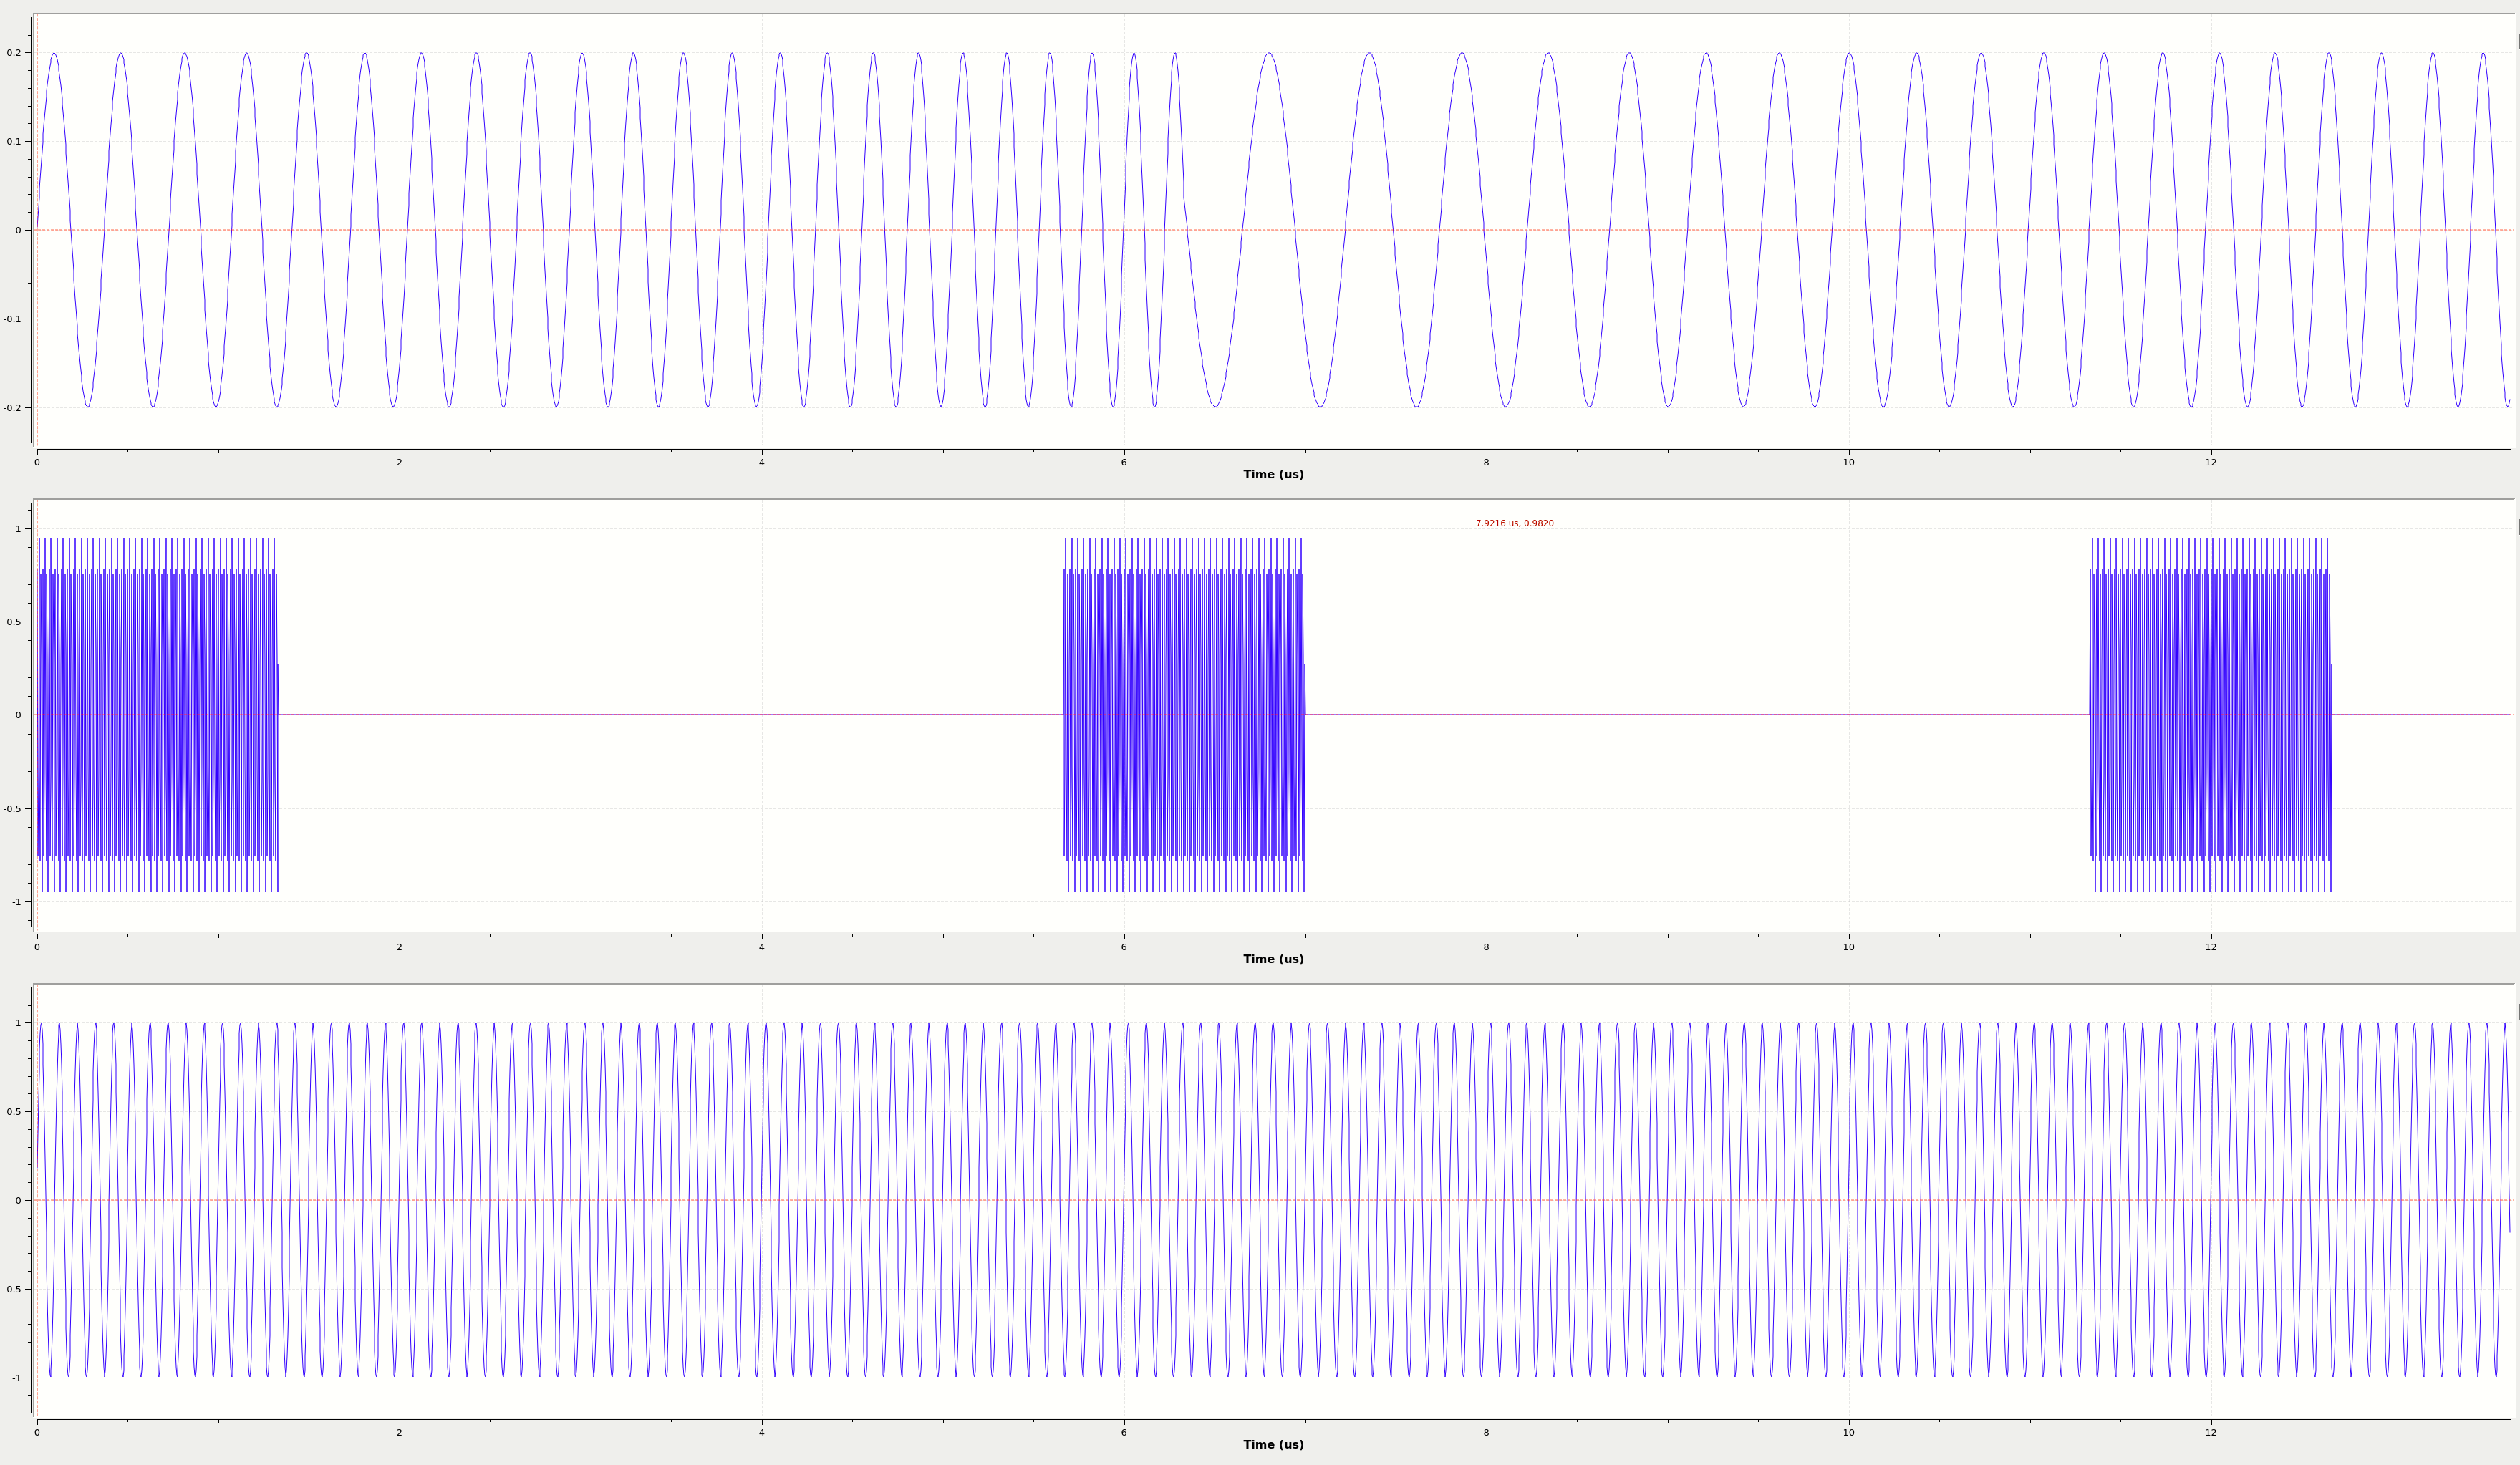
\includegraphics[width=1\textwidth]{Figures/radar_types.PNG}
    \caption{\ac{FMCW}, pulse \ac{CW}, and \ac{CW} radar}
    \label{fig:radar_types}
\end{figure}

%% Cognitive radar
% Contrast simple radar to modern stuff
\todojc{I do not understand this here, are you talking about what was mentioned before (surely not), or do you want to refer to what you are going to say next (if so rephrase)}\textbf{Such simple and somewhat contrived examples are obviously not representative of contemporary methods}, but indeed are they necessary in undertaking such fundamental and novel research, thus in order to fully \textbf{contrast this artificiality}, we look to "cognitive radar".
%%Cognitive Radars: A Reality?
% A definition
S. Haykin describes cognitive radar as one that "continuously learns about the environment through experience gained from interactions with the environment, the transmitter adjusts its illumination of the environment in an intelligent manner, the whole radar system constitutes a dynamic closed feedback loop encompassing the transmitter, environment, and receiver" \cite{haykin_cognitive_2006}.
% A second definition
Greco et. al. \cite{greco_cognitive_nodate} concur, but stress a distinction between adaptive and cognitive radar wherein the former is constrained to receive processing only, and the latter incorporating on-the-fly intelligent transmit characteristics.
% The need thereof
The authors' primary argument on behalf of cognitive radar is the lack of spectrum availability for traditional mono-function radars to operate.
% Comparison to other dense environment concerns
This mirrors earlier observations by M. Petterson:
\begin{quote}
    \textit{"The increased pulse density created by the deployment of pulse Doppler radar, both enemy and friendly, has created demand for systems with a high signal processing capability"}  \cite[p. 42]{pettersson_illustrated_1992}
\end{quote}
% Better <-> different <==> different => quantum (:. quantum -> better)
Either high signal processing capability or different signal processing capability are needed, and if a different capability is suitable for cognitive signal processing, then so too could a different approach work for quantum signal processing.

% Critique
% FIXME!
% Haykin presents a clear and evidenced to cognitive radar using probabilistic Bayesian models, with the ultimate goal of increasing signal-to-noise ratio (SNR). %(or signal-to-interference)

%% Chapter 3 - Foundations of cognitive radar for next-generation radar systems
% Cognitive radar definition (thesis)
N. A. Goodman \cite{goodman_chapter_2018} notes a historical trend in radar design wherein nearly every element of a radar system was defined by rigid, predefined patterns - in waveform design, signal processing, scan strategies, and more.
% Cognitive radar definition (antithesis)
Cognitive radar stands in polar opposition to this.
It is characterised by agile transmitted pulses, trainable signal processing, and intelligent scan strategies. 
% Relatio
Of particular interest in Goodman's work, is the principle of sequential hypothesis testing, whereby - similar to the scientific method - evidence is accumulated and beliefs are updated as new information becomes available.
% Comparison
They state two practical manifestations of this idea: Bayesian inference and \ac{POMDP}.

%% Bayesian
% input
Bayesian inference can be used to model the probability that a given signal comes from a specific source or emitter, given the available evidence or observations.
% process & ouptut
This involves constructing a prior probability distribution based on prior knowledge and assumptions about the signal and emitter characteristics, and then updating this distribution as new observations are obtained.
% Related research
Previously explored by Haykin \cite{haykin_cognitive_2006} and even earlier by Chair and Varshney \cite{chair_distributed_1988}, Bayesian inference is well-established in \ac{EW}, with later research by Matuszewski and Kawalec \cite{matuszewski_knowledge-based_2008} focusing specifically on a pure \ac{ESM} context.
% This is a hard problem
However, with current classical methods, this method is NP-hard. \cite{cooper_computational_1990}.
% Quantum has a solution!
There has been numerous studies on quantum-Bayesian models \cite{nimbe_models_2021}, which may hold promise to more efficient algorithms. 
Its applicability is unsurprising given the inherent probabilistic nature of quantum computing.

% POMDP
\ac{POMDP} was the second method in sequential hypothesis testing by Goodman, which intends to incorporate the incomplete knowledge of the signal environment with traditional \ac{MDP}'s.
% Complexity
While itself not isolated to radar signal processing, \ac{POMDP} is also challenging to solve on a classical computer, with Bernstein et al. finding it PSPACE-hard \cite{bernstein_complexity_2002}.
% Quantum complexity
\todo{This needs to be confirmed.} Interestingly, Barry et al. \cite{barry_quantum_2014} found that, not only does a quantum \ac{POMDP} policy exist, but it may have at least the same complexity as their classical counterparts.

% Other methods
There are a few other notable \ac{ESM} methods.
% Hardware (FPGA) Real-time radar pulse parameter extractor
Iglesias et al. \cite{iglesias_real-time_2014} present a parameter estimation of \ac{TOA}, \ac{PW}, frequency, power, and \ac{SNR} in a \ac{FPGA}.
Their research provides a baseline performance level of conventional classical methods to which any quantum methods must strive to meet.
% Wavelet method
Ehara et al. \cite{ehara_weak_1994} present a similar such reference point, but yield some insights on how wavelet transforms can be used as a preprocessing transform for further signal analysis.
The wavelet method has particular relevance to radar as it can represent both the time-variant and frequency-variant nature of radar signals.
% Quantum equivilent
More relevant to this study however, is research by Høyer \cite{hoyer_efficient_1997} where quantum wavelet transforms are presented.


% Wigner-Hough-Radon transform
Another pre-process that has been used for \ac{ESM} signals is the Wigner-Hough-Radon transform \cite{gulum_parameter_2012}, that translates time and frequency information into a parameter space.
% Application to radar
The work of Gulum et al. found specific and performant applications to \ac{FMCW} radar.
% Quantum equivilency
Importantly, recent research by Ma et al. \cite{ma_quantum_2021} has found a quantum equivalent to the closely related Radon transform, finding an exponential speedup for applications in image signal processing.

% Object Recognition and Identification Using ESM Data
% Link to from many techniques to need for fusion
Taghavi et al. \cite{taghavi_object_2016} propose that - while useful in isolation - these same methods can be even more performant when fused with kinematic measurements (i.e., of position and velocity). 
% Goal their research
The ultimate goal of their research to develop a framework for recognising and identifying maritime targets of interest using this data fusion approach.

% Deinterleaving of radar signals and PRF identification algorithms
Similar to Taghavi et al. \cite{taghavi_object_2016}, A.W. Ata'a and S.N. Abdullah \cite{alhashimi_deinterleaving_2007} cluster data in both kinematic (\ac{DOA}) and signal parameter (\ac{RF}) domains using a self-organising neural network named 'Fuzzy ART', with the end goal of deinterleaving radar signals.
% Goal and result
The Fuzzy ART approach yielded effective results, with the authors finding the average clustering quality of 0.826 with an average deviation of 6.47\% (r=0.88, n=1000), and accurate classification of up to 100 emitters.
% Simulated data => Generalisability
Both A.W. Ata'a and S.N. Abdullah, and Taghavi et al. use simulated data generated using software
and consequently raises doubts as to the generalisability of their results, since simulated data may not accurately reflect real-world conditions.
% Bigger problem of source data
More broadly, highlights a more systemic challenge in radar signal analysis research.
% Inherent to the problem: not methodological
Although the lack real-world sample data has been observed in other studies \cite{svensson_classification_2022, noone_neural_1999, mason_deep_2017}, it may not necessarily reflect a widespread methodological failure.
% Inherent to the data
Rather, it could be considered an inherent consequence of the numerous degrees of freedom, limited accessibility to sample emitters, and difficulty in isolating the independent variables of \ac{ESM} signals.

\subsection{ML for Radar Signal Processing}
% Nature of data suited to ML
The complex and high-dimensional nature of radar signals has led to the use of \ac{ML} methods, such as \ac{ANN} and \ac{kNN}. 
% Research which capitalises on such a trait
A. Svensson \cite{svensson_classification_2022} presents a survey of several approaches in specific applications to \ac{EW} and \ac{ESM}; classification of emitters based on \ac{PRI}.
% Svensson's methods:
The author applies two feature extraction techniques: \ac{PCA} and Wavelet Transforms to the radar signals.
% Results
Experimentally, Svensson's methods yielded between 96\% - 98\% classification accuracy, however the study used simulated (yet restricted access) data. 
% Bias, but good enough
Disregarding any potential bias and reproducibility constraints imposed by their commercial interest, the study shows that \ac{ML} methods are feasible and practically relevant.

% \todo{ Knowledge-based}
% \todo{    - Knowledge-based Signal Processing for Radar Identification}
% \cite{matuszewski_knowledge-based_2008}
\todo{ ML: Basic techniques}
\todo{    - Classification of Radar Emitters Based on Pulse Repetition Interval using Machine Learning}
\todo{ Machine learning (survey)}
\todo{    - Deep-Learning for Radar: A Survey}

% Link to aforementioned research
Neural network reinforcement learning was noted by Haykin \cite{haykin_cognitive_2006} as "best suited" to cognitive radar systems.
% Older than Haykin. Initial research by Noone; many more since.
G.P. Noone \cite{noone_neural_1999} initially explored the concept of neural networks to detect modulation, but countless papers have since been published across many applications in \ac{ESM}:
% Survey
Mason et al. \cite{mason_deep_2017} provide a broad outlook on the current state of affairs in the use of deep learning in radar signal processing.
The authors analysed a large body of research over several areas of radar signal processing and for a multitude of deep learning techniques with varying degrees of effectiveness:
\begin{itemize}
 \item \todojc{Are they all relevant to radar signal processing? If so briefly state how}CNN: Convolutional neural network
 \item DBN: Deep belief network
 \item DRL: Deep reinforcement learning
 \item DRES: Deep residual neural network
 \item FNN: Feed-forward neural network
 \item GAN: Generative adversarial network
 \item RNN: Recurrent neural network, including long-short term memory
 \item SAE: Stacked auto-encoder
\end{itemize}

Several limitations were also identified, some being systemic to the field, others specific to deep learning techniques.
Once challenge identified was \todojc{What does it mean?} \ac{DNN}'s \textbf{subjectivity to Electronic Attack (EA)}, where, depending on the level of intelligence about the specific \ac{DNN} techniques employed, various exploitations may be executed.
Of course, EA is not specific to DNN's, however, it's noted that because they exist as an heuristic model, they necessarily have gaps in their model of the problem space.
Therefore, it's noted that DNN's may be more susceptible to EA because of its inherent non-analytical method.

Again, the lack of training data was identified as a serious limitation (especially for \ac{DNN}'s, that require large amounts of training data).
The paper concludes with an evaluation of particularly effective methods, some reaching > 97\% accuracy, albeit with small training sample sizes.

% The primary interest of \todojc{which option? DNN?}\textbf{this option} is in passive radar, i.e., radars which generally do not transmit energy and listen to a return. An example is a Radar Warning Receiver (RWR) which is a passive electronic warfare support system \cite{avionics_department_electronic_2013}

% One functional mode of RWR's is the search mode: where the system’s objective is to interrogate the electromagnetic environment to detect and identify emitters. The only information that radars are given is the signals which it receives, and its location in space and time (as well as some prior understanding of the operational environment). Due to the nature of the operating context, modern radars may receive many incident signals in a short period of time. Within such received signals, there may exists a number of constituent parts: communications signals, radar signals, interference (whether intentional or not), and noise (being environmental, or system). For signals originating from radars, they vary in several dimensions: see radar domains. Noise is generally constant, but limits the receiver’s ability to detect a given signal’s presence. Interference is any signal which interferes with the receiver’s ability to perform its function – either fully or partially. The functional operation of the receiver is: signal input (coming from antenna), RF front-end, digitisation, and processing. In each stage, the signal may change characteristics and formats based on a variety of filtering and processing operations. \cite{stimson_introduction_1998}\todo{This last one needs to be refined and specified to more constraints / trade-offs of radar I think.}
\todo{ DNN: }
\todo{    - A Complete Framework of Radar Pulse Detection and Modulation Classification for Cognitive EW}
\todo{ DNN - recurrent}
\todo{    - Classification, Denoising, and Deinterleaving of Pulse Streams With Recurrent Neural Networks}

\subsection{Quantum Technology for Radar Signal Processing}

%%%%%%%%%% Begin Quantum:

% Vast...
From Bayesian inference to \ac{MDP}'s; mathematical transforms to heuristic methods and \ac{ML} - classical radar signal processing is vast and diverse.
% but insufficient
Yet, while many methods are effective, they often require a trade-off between accuracy and computational complexity.
% .: quantum computing could be the solution
Therefore, given these considerations, quantum computing is a candidate solution that warrants further investigation.

%% Qubits
% Qubits seem to be multi states
Quantum computing operates on qubits, which, from a classical perspective, may seem to exist in multiple states at once.
% More a result of quantum nature; a different category/domain
However, this is more a result of the principles of superposition and entanglement, which allows for a different type of state representation in the quantum domain.
% Measurement => transformation
Through classical measurement, this quantum state can be observed and thereby transformed back to the classical domain, but the underlying quantum state is fundamentally different from classical states.
% Gates & mathematical representation
Computation is affected by gates, where qubits are manipulated using quantum operations represented mathematically by unitary matrix operators acting on a Hilbert space.
% Circuits made from gates => potential exp. speedup
Through the repeated application of these gates, quantum circuits can be constructed to perform complex computations, which, in some cases, may exponentially faster than classical implementations.

% The principle is old; but now standardised
Quantum computation goes back to R.P. Feynman from 1981 \cite{feynman_simulating_1982}, subsequent work has since formalised it into a standardised model of computation.
% Quantum universality
Such efforts in standardisation took a leap forward thanks to work done by D. Deutsch's \cite{deutsch_quantum_1985} in 1985 on the universality of a quantum computing machine.
% Quantum computer implementations
Practical computation is now possible using both simulated \cite{noauthor_quantum_nodate, noauthor_simulators_nodate} and physical machines \cite{noauthor_ibm_2015, noauthor_microsoft_nodate}, the latter computers being termed '\ac{NISQ} machines'.
% Quantum programming languages
There also now exists over a dozen programming languages and numerous research groups \cite{garhwal_quantum_2021} in the quantum computing domain.
% SDK's exists
Several software development packages have also been developed that present many of these functions to a quantum software developer.
% Examples
Some examples are Qiskit \cite{qiskit_contributors_qiskit_2023}, and PennyLane \cite{noauthor_pennylane_nodate}.

% Quantum time series
Quantum computing has been used to solve a variety of problems, but the principal focus of this examination is on quantum signal processing and the prerequisites thereof.
% Encoding patterns for quantum computers
Weigold et al. \cite{weigold_encoding_2021} details several techniques for encoding data for quantum algorithms.
The problem presented in the paper, similar to that of Daskin's remarks, is that while quantum computing may be in superior to classical methods in solving some problems, it is data loading which is often found to be inefficient and ineffective.
Therefore, after starting with a description of the quantum computing mechanism in general, the paper proceeds to present an enumeration and comparison of various means of transforming data into the Hilbert space:

\begin{itemize}
 \item Basis encoding
 \item Angle encoding
 \item QuAM encoding 
 \item QRAM encoding
 \item Amplitude encoding
\end{itemize}

Weigold et al. comprehensively detail each approach, its applications, methods, and variants.
Interestingly, the authors also present four methods on preprocessing - with much overlap to work by Daskin \cite{daskin_walk_2022}:

\begin{itemize}
 \item Schmidt decomposition
 \item Matrix encoding
 \item Quantum Phase Estimation
 \item Post-selective measurement
\end{itemize}

Overall, the paper presents a survey of encoding approaches with strong analytical grounding; the paper effectively describes and identifies the benefits and limitations of each encoding method in terms of efficiency and entropy conversion trade-offs.
However, while the approaches mentioned soundly apply to various forms of classical data, the authors do not demonstrate their methods with a diverse range of real-world data. 
A specific example of interest to this research is multivariate time-series data, which is not yet represented faithfully by quantum computing, nor indeed by classical computing methods.

% A walk through of time series analysis on quantum computers
A. Daskin \cite{daskin_walk_2022} explores this such topic, presenting a systematic and comprehensive survey of a number of fundamental techniques in quantum time-series analysis.
% State prep.
Daskin notes that in order for temporal data to be processed by a quantum computer, it must first be mapped from its classical representation to a vector defined in the Hilbert space.
% Preprocessing
After this, the data then may be preprocessed (in the quantum domain), in order that subsequent quantum computation may be performed - in Daskin's research, this was time-series forecasting.
% Challenge
In concluding their research, the author makes an apt note regarding the challenges of quantum time-series analysis:
\begin{quote}
    \textit{As future direction, more example data analysis are needed to investigate algorithms and methods for preprocessing and transformation of time series data into the Hilbert space in which quantum computers work better than classical computers.} \cite{daskin_walk_2022}
\end{quote}

% Evaluation of encoding
Evaluating the quantum encoding method is also important, and will be partially the subject of this enquiry.
% Expressibility and Entangling Capability of Parameterized Circuits for Hybrid quantum/classical Algorithms
In their paper on the subject, Sim et al.\cite{sim_expressibility_2019} propose that since many quantum algorithms rely on an objective function derived from parameterised quantum circuits, the accuracy and scalability of these algorithms are dependent on the fidelity of the parameterisation, or the "expressive power" of the quantum circuit.
% Therefore expressibility is good
Therefore, achieving a satisfactory representation of the input space in the Hilbert space is important.
Sim et al. also describe the entanglement capability of parameterised circuits, and how that too is important when calculating over multiple states at once.
% Expressibility is bounded by circuit cost
The authors also note that although expressibility is good as an ends, it is constrained in performance by the means of achieving it - quantum gates.
More specifically the circuit cost: depth, connectivity, and number of parameters.
% Relevance
This is relevant to any future quantum solution to \ac{ESM} signal analysis, as highly expressive quantum circuits tend to perform better and can mitigate barren plateaus.

% Survey of algorithms themselves
Nimbe et al. \cite{nimbe_models_2021} present a broader survey of quantum models in their systematic review of the subject - each approach having potential to be used as a technique for \ac{ESM} signal analysis:
\begin{enumerate}
    \item Circuit models
    \item Quantum perceptron
    \item Quantum automata
    \item Quantum neural computation and \ac{QNN}
    \item Algorithms based on the \ac{QFT}
    \item Quantum image restoration algorithms 
    \item Quantum Bayesian statistics and inference
    \item Quantum information processing
\end{enumerate}

% Partitio
Of these, \ac{QNN}, quantum Bayesian inference, and \ac{QFT} methods - all fundamentally facilitated by circuit models - show the most promise for radar signal analysis.
% Bayesian method already explored, and somewhat QFT methods (Wavelet transform), will turn to QNN's.
Discussed previously were methods for quantum Bayesian inference, statistical methods based on \ac{MDP}'s \cite{barry_quantum_2014}, and Fourier analysis \cite{hoyer_efficient_1997, fijany_quantum_1998} therefore \ac{QNN}'s are looked to next.
% Analogue for DNN
\ac{QNN}'s have a direct analogue to classical techniques: neural networks.
% Classical NN's good => QNN's good too?
Classical neural networks have proven effective in radar signal processing \cite{noone_neural_1999, haykin_cognitive_2006, mason_deep_2017, liu_classification_2019} and therefore experiments in \ac{QNN}'s are a vauable endevour, as little research has been done on the subject.

% QNN's description
According to Schuld et al. \cite{schuld_quest_2014} \ac{QNN}'s begin by encoding data into an initial quantum state, and after having done quantum operations on it, produce a stable output which is closest to the input given some distance measure.
It should also, according to the authors, exhibit at least one neural computing mechanism, and be consistent with the tenants of the quantum computing paradigm.

% Complex: recurrent
More complex iterations of quantum neural networks are seen in work by Takaki et al. \cite{takaki_learning_2021}
% Classical corrospondent
This is directly relevant to research by Liu and Yu \cite{liu_classification_2019} on classical recurrent neural networks.

% Resource management
Finally while the scope of this paper does not permit a complete exposition of all the ways quantum computing may be applicable to \ac{EW}, it is noted that quantum computing may be applied to non-signal processing applications, such as resource management \cite{charlish_autonomous_2011, charlish_development_2020}.

\subsection{Gap-analysis}

% Summary
In the context of radar signal processing, quantum computing has emerged as a promising option, offering the potential to overcome the limitations of the classical approaches (see Figure \ref{Fig:conceptual_model}).

\todojc{Text in diagram not readable Also note that any figure needs a description in text, and so would the model}
\begin{figure}
    \centering
    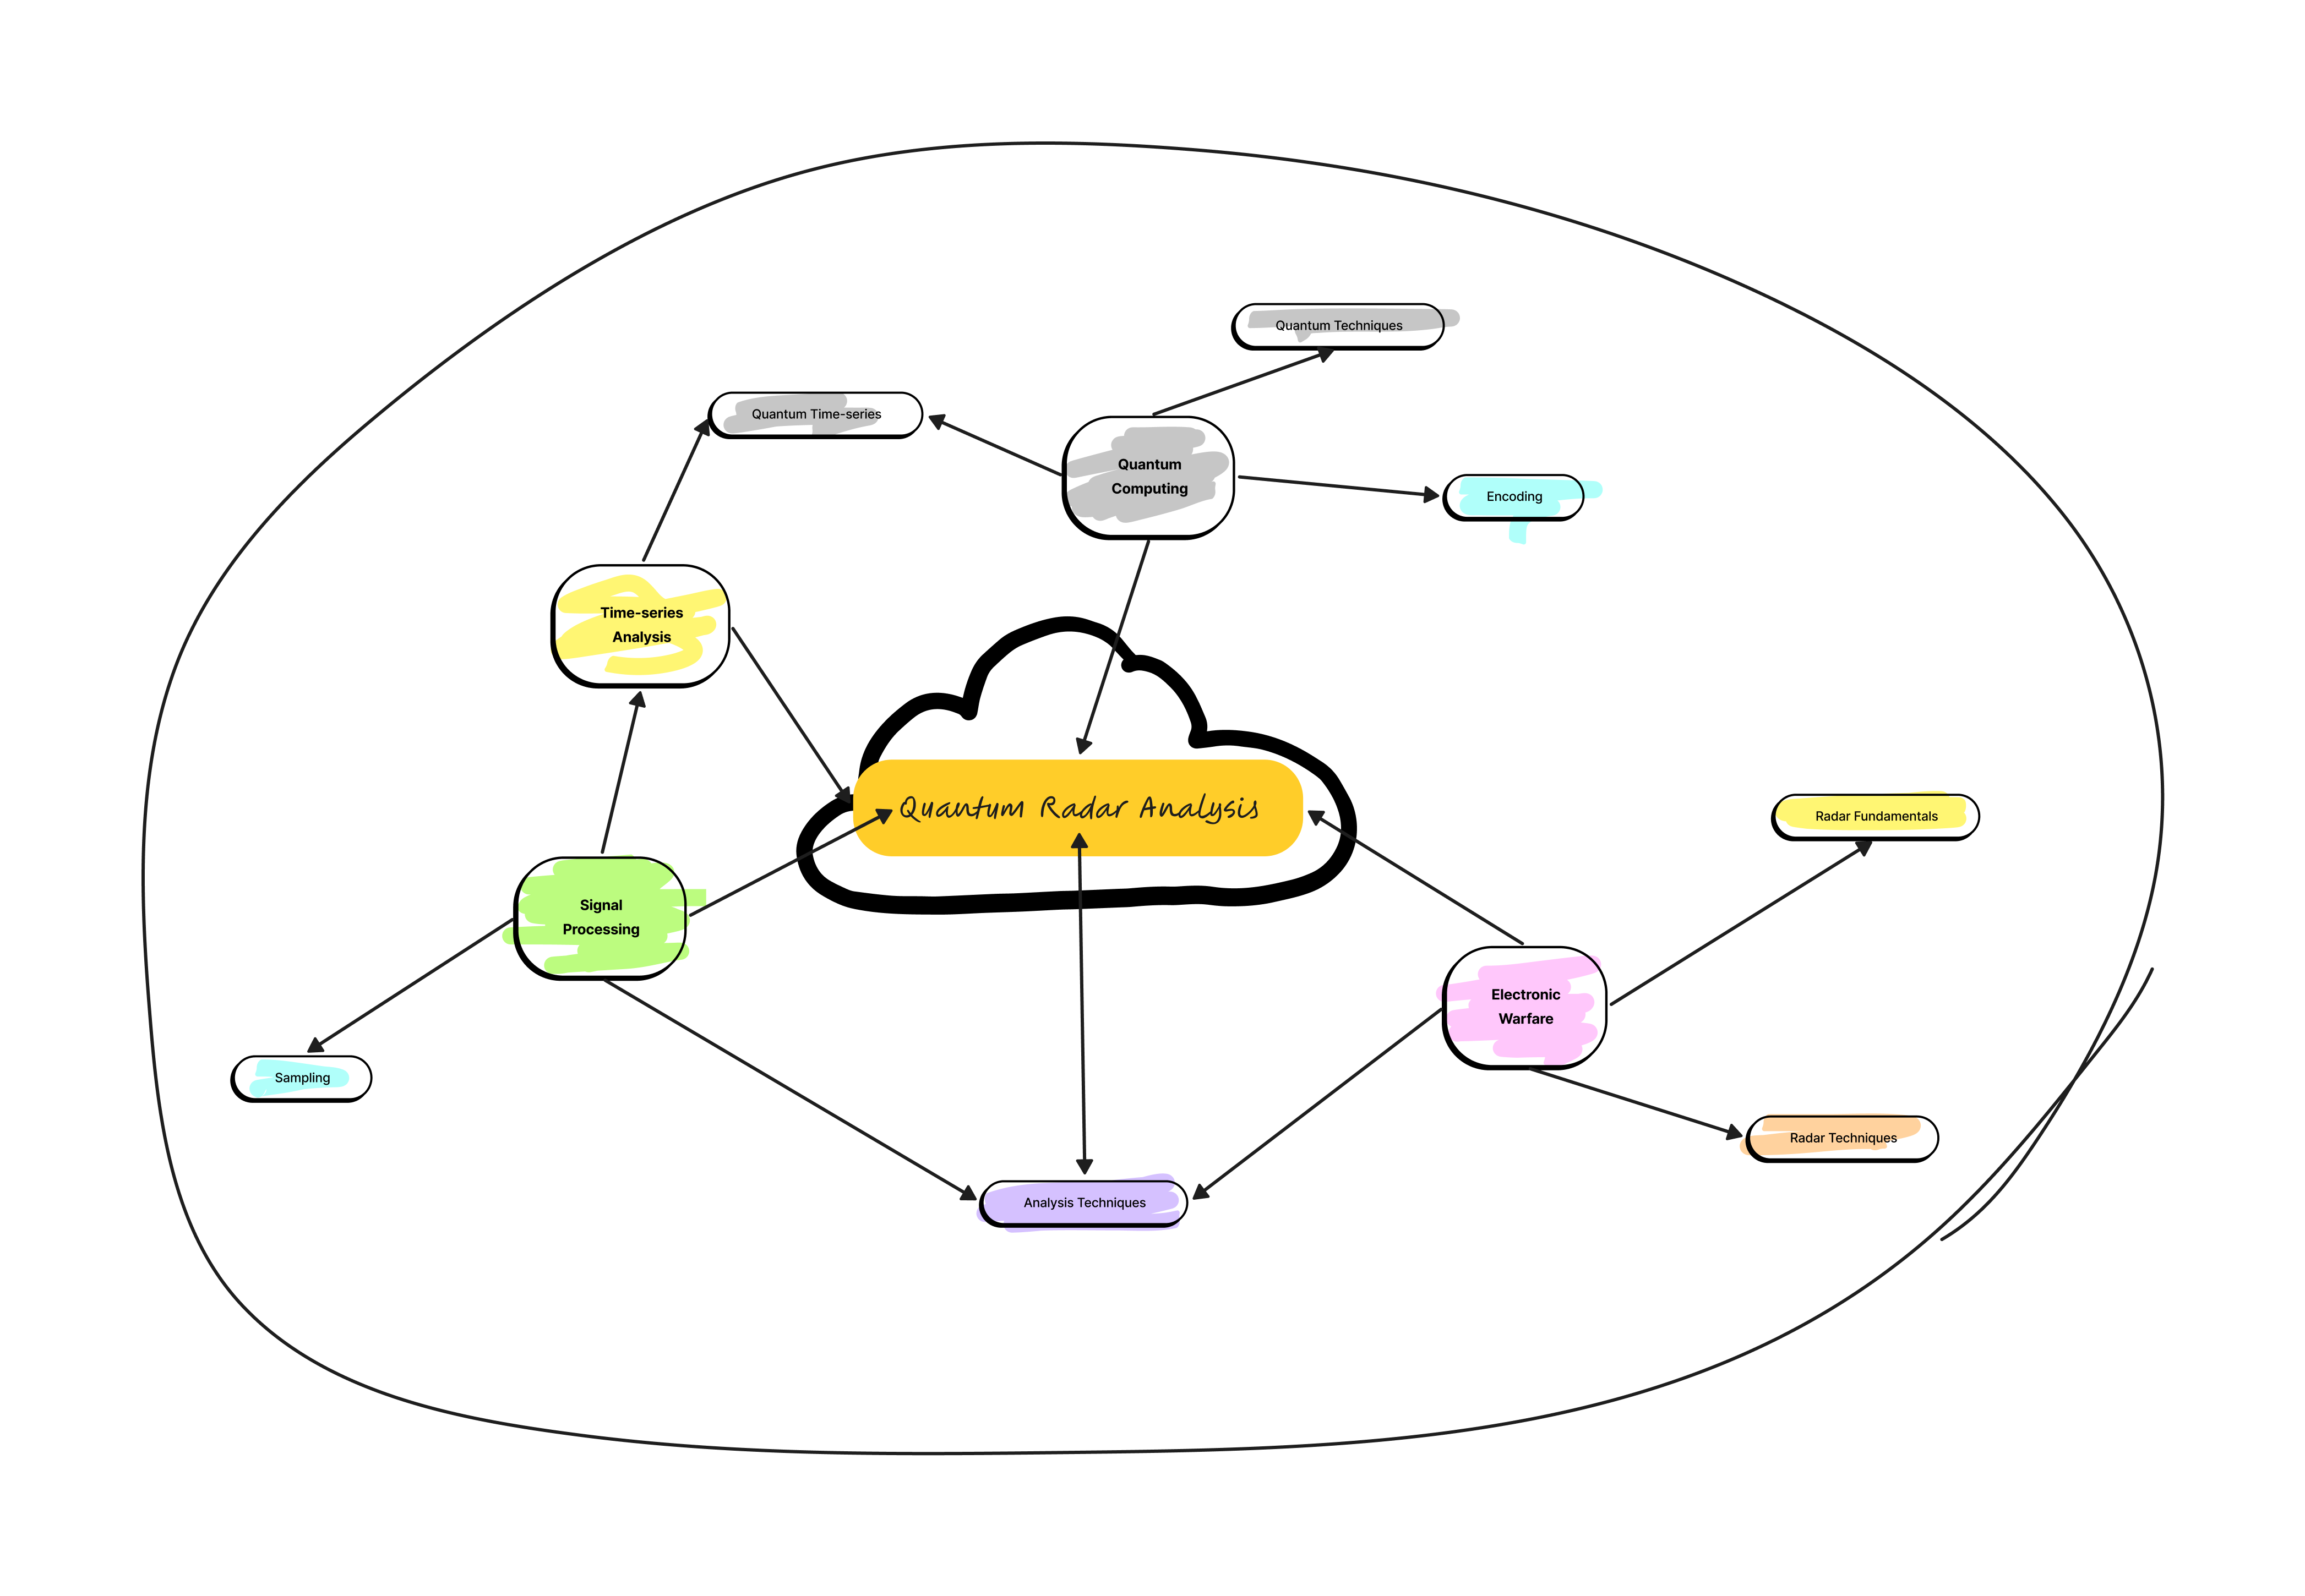
\includegraphics[width=1\textwidth]{Figures/Literature review - mind map.png}
    \caption{The conceptual model for the study}
    \label{Fig:conceptual_model}
\end{figure}

% Quantum
\todojc{As you talk about the "gap" refer to and discuss what is in the "conceptual model"}A large body of research has been conducted into quantum computing, with many papers focusing on quantum problem solving methods and encoding.
Furthermore, the realm between that, and of signal processing have been explored to a lesser degree.
However, the niche of encoding time-series sampled data (as what will be required in this research) has only been explored in more limited respect.
From the perspective of method, many studies in quantum computing were found to lack methodological precision.

% Radar
The field of radar too has been extensively explored over many previous decades.
Many studies have explored the fine details of radar techniques, few studies clearly defined simpler approaches in radar.
While there is a wealth of literature on radar processing, the gap exists not in the field as it stands, however in the lack of contra-normative methods, like quantum computing.
It was also seen that the body of accessible literature was notably lacking in valid, diverse, and accessible source data.

Given these insights, it was found that little available research exists on the fusion of radar/\ac{EW}, signal processing, and quantum computing - despite large bodies of research existing in each respective field alone.
Therefore this combination is the line of enquiry this research will address.
% Additionally, this study aims to address the general deficiency in methodological rigor, of which both principal areas of interest were found to lack.

% NOTES FROM MEETING 1
% 1. Academic references - explain / summarise them\\
% 2. Develop a meta-model of their fundamental argument, challenges, deficiencies, and strengths\\
% 3. Compare their differences, similarities, and whether or not they agree. (If they all agree, more sources should be found); how they interrelate.\\
% 4. Next, the exposition of the problem space (radar signal analysis) should be written, being lean enough so as to only explain the content of the referenced academic sources. I.e., the challenges faced should be fully developed.\\
% 5. Following which, a more precise formulation of problems should be undertaken.

% Here are some ones I would like to properly analyse in more depth (not yet added to Zetaro)
% - https://ietresearch.onlinelibrary.wiley.com/doi/pdf/10.1049/iet-rsn.2017.0516
% - https://ietresearch.onlinelibrary.wiley.com/doi/pdf/10.1049/iet-rsn.2017.0563
% - Improvements on deinterleaving of radar pulses in dynamically varying signal environments: Kenan Gençol, Ali Kara, Nuray At (2017)
% - Estimating the Instantaneous Frequency of Linear and Nonlinear Frequency Modulated Radar Signals — A Comparative Study Hubert Milczarek, Czesław Le´snik, Igor Djurovi, and Adam Kawalec
